
	\section{植物细胞}
	
	\subsection{植物细胞的形状和大小}
	
	植物细胞的形状多样,与其功能相适应。(\autoref{fig:植物细胞的多种形态})
	
	\begin{figure}[htbp]
		\centering
		\includegraphics[width=\linewidth]{Pics/植物细胞的多种形态}
		\caption{植物细胞的多种形态}
		\label{fig:植物细胞的多种形态}
	\end{figure}
	
	
	为了保持较大的相对表面积,细胞通常很小。特例有番茄、西瓜的“果肉”(细胞较大),棉的表皮毛、麻的纤维(仅前后径较长)等。
	
	\subsection{植物细胞的结构与功能}
	
	植物细胞的基本结构如\autoref{fig:植物细胞的结构划分}所示。
	
	\begin{figure}[htbp]
		\centering
		\begin{forest}
			forest scheme
			[植物细胞
				[细胞壁
					[胞间层]
					[初生壁]
					[次生壁]]
				[原生质体
					[原生质膜]
					[细胞核]
					[细胞质
						[细胞质基质]
						[细胞器(质体、液泡等)]
						[后含物(淀粉粒等)]]]]
		\end{forest}
		\caption{植物细胞的结构划分}
		\label{fig:植物细胞的结构划分}
	\end{figure}
	
	\subsubsection{细胞壁}
	
	\paragraph{细胞壁的层次}
	
	细胞壁的位置、化学成分等见\autoref{tab:细胞壁的层次}。
	
\begin{table}[htbp]
	\zihao{5}
	\centering
	\begin{tabularx}{\textwidth}{|c|c|c|C|c|}
		\hline
		\textbf{细胞壁} & \textbf{位置} & \textbf{特点} & \textbf{化学成分} & \textbf{功能} \\ \hline
		胞间层(中层) & 外 & 薄、可塑 & 果胶 & 彼此粘连 \\ \hline
		初生壁 & 中 & 薄,可塑 & 纤维素、半纤维素、果胶、结构蛋白 & 支持、保护 \\ \hline
		次生壁 & 内 & 厚、坚硬 & 半纤维素、纤维素、木质素 & 支持、保护 \\ \hline
	\end{tabularx}
	\caption{细胞壁的层次}
	\label{tab:细胞壁的层次}
\end{table}
	
	细胞壁中含有的物质如下列:
	\begin{description}
		\item[纤维素] 多糖,Glc残基以$\beta$-1,4糖苷键连接,组成微纤丝、大纤丝;
		\item[半纤维素] 支链与纤维素不同,按照支链的不同可分为双子叶植物中的\sy{木葡聚糖}和单子叶植物中的\sy{阿拉伯木聚糖};
		\item[胼胝质] Glc残基以$\beta$-1,3糖苷键连接的多糖,能应对机械损伤和病虫害。可由间苯二酚蓝显色;
		\item[果胶] 双子叶植物多,单子叶植物很少;
		\item[木质素] 疏水的酚醛聚合物(非糖类)。可被盐酸-间苯三酚染色。
		\item[蛋白质] 主要是结构蛋白和酶。结构蛋白包括富含羟脯氨酸、脯氨酸、甘氨酸的三类。其中富含羟脯氨酸的蛋白就是伸展蛋白。
	\end{description}
	
	除此之外,细胞壁中还随功能不同,含有角质、栓质、矿质等。
	
	细胞壁的结构单位是\sy{微纤丝}。微纤丝是一种纤维素的构架,层次有:
	\begin{center}
		葡萄糖$\longrightarrow$葡萄糖长链$\longrightarrow$微团$\longrightarrow$微纤丝$\longrightarrow$大纤丝(光镜下可见)
	\end{center}
	
	初生壁的微纤丝排列成网状,三层次生壁中微纤丝排列各不相同。细胞壁的其他物质就填充在微纤丝骨架中。
	
	初生壁中,三类物质的作用分别是:
	\begin{description}
		\item[果胶] 构成基质,如同水泥;
		\item[纤维素] 构成支持部分,如同钢筋;
		\item[半纤维素] 靠氢键交联果胶和纤维素。
	\end{description}
	
	次生壁中,需要注意:
	\begin{itemize}
		\item 并非所有细胞都有次生壁;
		\item 次生壁的3层结构中,微纤丝排列方向不同是纤维素合成酶的排列方向由微管排列方向决定的缘故;(\autoref{fig:植物细胞壁的不同层次和微纤丝的排列方向})
		\item 大多数具有次生壁的细胞均死亡。
	\end{itemize}
	
	\begin{figure}[htbp]
		\centering
		\includegraphics[width=0.4\linewidth]{Pics/次生壁的3层}
		\caption{植物细胞壁的不同层次和微纤丝的排列方向}
		\label{fig:植物细胞壁的不同层次和微纤丝的排列方向}
	\end{figure}
	
	\subsubsection{初生纹孔场与胞间连丝}
	
	初生壁上细胞壁较薄的区域称为初生纹孔场,这里分布许多小孔,有胞间连丝穿过。
	
	胞间连丝是沟通相邻细胞的原生质细丝,外有内质网形成的管道。胞间连丝并不局限于初生纹孔场。
	
	\subsubsection{纹孔}
	
	\sy{纹孔}是初生壁上没有被次生壁覆盖的部分。按照次生壁在此处的加厚特点,分为单纹孔\footnote{这里的“单”指的是简单(simple),意思是结构比较简单的一种纹孔。}和具缘纹孔。(\autoref{fig:纹孔})
	
	\begin{itemize}
		\item 具缘纹孔与单纹孔的区别就是具缘纹孔的次生壁向细胞内拱起,使纹孔腔变大。
		\item 某些裸子植物的具缘纹孔还具有纹孔塞,可控制水流。
	\end{itemize}
	
	\begin{figure}[htbp]
		\centering
		\includegraphics[width=\linewidth]{Pics/纹孔}
		\caption{纹孔}
		\label{fig:纹孔}
	\end{figure}
	
	\subsubsection{液泡}
	
	液泡由高尔基体起源。随着细胞成熟,液泡从小而分散变为大而集中。
	
	液泡内有细胞液,起到储存、防御、膨压、消化的作用。
	
	液泡可吞噬衰老细胞器,起到动物的溶酶体的功能。这一功能是由液泡膜整合蛋白(TIP)决定的。若TIP为$\gamma$型,则该液泡承担溶酶体的功能。
	
	液泡压缩了原生质的体积,相当于节省了氮元素。
	
	\subsubsection{质体}
	
	质体是植物细胞特有的细胞器之一,与糖类的合成与贮藏密切相关。
	
	按照含有色素的种类,分为:
	\begin{description}
		\item[叶绿体] 含有叶绿素、叶黄素、类胡萝卜素。进行光合作用。基质内有基粒。
		\item[有色体] 含有胡萝卜素、叶黄素。存在于果实、花瓣中。聚积淀粉和脂质,吸引传粉、传种动物。无基粒。
		\item[白色体] 不含色素。储存淀粉(淀粉体)、脂肪(造油体)。无基粒。
	\end{description}
	
	
	质体都由前质体发育而来,具体转变如\autoref{fig:质体的转化}所示。
	
	\begin{figure}[htbp]
		\centering
		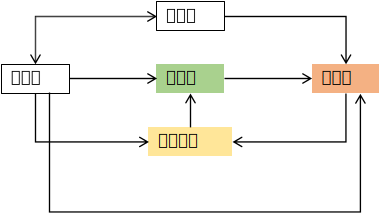
\includegraphics{质体的转化}
		\caption{质体的转化}
		\label{fig:质体的转化}
	\end{figure}
	
	三种成熟质体可以互相转化,除了叶绿体不能转化为白色体。
	
	\sy{黄化质体}中含有原片层小体,是管状的膜系统,见光之后迅速发育为叶绿体的类囊体。
	
	\subsubsection{微体}
	
	微体与溶酶体相似,区别是二者含有的酶不同。溶酶体含有水解酶类,微体含有氧化酶和过氧化氢酶。
	
	微体分为过氧化物酶体和乙醛酸循环体。动物没有乙醛酸循环体。
	
	\subsection{植物细胞的后含物}

	 后含物是细胞原生质体新陈代谢产物,包含贮藏物和废物,化学上包括糖类、蛋白质、脂质、无机盐和其他有机物。后含物存在于原生质体或细胞壁。
	 
	 下面介绍常见的后含物,包括淀粉、蛋白质、脂肪、晶体。
	 
	 \subsubsection{淀粉}
	 
	 淀粉主要以\sy{淀粉粒}的形式存在。
	 
	 \begin{itemize}
	 	\item 合成过程:
	 	\begin{itemize}
	 		\item 由质体合成,白色体特化为造粉体;
	 		\item 沉积方式:由脐点逐层向外沉积;
 			\item 脐点位置决定类型:同心淀粉、离心淀粉。
	 	\end{itemize}
	 	\item 结构特征:
	 	\begin{itemize}
	 		\item 轮纹结构:直链淀粉与支链淀粉交替沉积;
	 		\item 光学差异:直链淀粉亲水性更强。
	 	\end{itemize}
	 	\item 形态分类(\autoref{fig:淀粉粒的类型}):
	 	\begin{itemize}
	 		\item 单粒淀粉粒:单脐点+同心轮纹;
	 		\item 复粒淀粉粒:多脐点+独立轮纹;
	 		\item 半复粒淀粉粒:多脐点+共同外围轮纹。
	 	\end{itemize}
	 \end{itemize}
	 
	 \begin{figure}
	 	\centering
	 	\includegraphics[width=0.3\linewidth]{Pics/淀粉粒的类型}
	 	\caption{淀粉粒的类型}
	 	\label{fig:淀粉粒的类型}
	 \end{figure}
	 
	 \subsubsection{蛋白质}
	 \begin{itemize}
	 	\item 贮藏形式:
	 	\begin{itemize}
	 		\item 蛋白质拟晶体:方形(如马铃薯块茎细胞)
	 		\item 糊粉粒:
	 		\begin{itemize}
	 			\item 结构:膜包裹的球状颗粒;
	 			\item 组成:无定形蛋白(+拟晶体),蓖麻种子的还含磷酸盐球形体(\autoref{fig:蓖麻的糊粉粒});
	 			\item 分布:胚乳糊粉层(豆类子叶细胞典型)
	 		\end{itemize}
	 		
	 		\begin{figure}[htbp]
	 			\centering
	 			\includegraphics[width=0.5\linewidth]{Pics/蓖麻的磷酸盐球形体}
	 			\caption{蓖麻的糊粉粒}
	 			\label{fig:蓖麻的糊粉粒}
	 		\end{figure}
	 		
	 	\end{itemize}
	 	\item 动态变化:
	 	\begin{itemize}
	 		\item 形成:液泡分裂$\longrightarrow$蛋白沉积$\longrightarrow$形成糊粉粒;
	 		\item 利用:糊粉粒分解$\longrightarrow$液泡重组。
	 	\end{itemize}
	 \end{itemize}
	 
	 \subsubsection{脂肪和油类}
		基本特征:
	 	\begin{itemize}
	 		\item 高能贮藏物质,体积最小
	 		\item 物理状态区分:常温固态为脂肪,液态为油类
	 	\end{itemize}
	 	
	 	质体和圆球体都能积累脂质,成为油滴。
	 
	 \subsubsection{晶体}
	 
	 \begin{itemize}
	 	\item 基本特征:
	 	\begin{itemize}
	 		\item 无机盐结晶,主要存在于液泡
	 		\item 草酸钙晶体为主
	 		\item 意义:降低次生代谢物毒性
	 		\item 特殊类型:碳酸钙晶体(钟乳体)
	 	\end{itemize}
	 	\item 形态分类(\autoref{fig:晶体的类型}):
	 	\begin{itemize}
	 		\item 单晶:棱柱状/锥状
	 		\item 针晶:针状聚集体
	 		\item 簇晶:球状复式结构
	 	\end{itemize}
	 	
	 	\begin{figure}[htbp]
	 		\centering
	 		\includegraphics[width=0.5\linewidth]{Pics/晶体的类型}
	 		\caption{晶体的类型}
	 		\label{fig:晶体的类型}
	 	\end{figure}
	 \end{itemize}
	 
	\section{植物的组织}
	
	\begin{figure}[htbp]
	\centering
	\begin{forest}
		forest scheme
		[植物组织
		[分生组织
		[按来源分
		[原分生组织]
		[初生分生组织]
		[次生分生组织]]
		[按位置分
		[顶端分生组织]
		[侧生分生组织]
		[居间分生组织]]]
		[成熟组织
		[保护组织]
		[薄壁组织]
		[机械组织]
		[输导组织]
		[分泌组织]]]
	\end{forest}
	\caption{植物的组织分类}
	\label{fig:植物的组织分类}
	\end{figure}
	
	\subsection{分生组织}
	
	如\autoref{fig:植物的组织分类}所示,分生组织可按两种不同的方式区分,而这两种方式是互相重叠的:(\autoref{fig:分生组织的分类})
	
	\begin{figure}[htbp]
		\centering
		
\includegraphics{分生组织的分类}
		\caption{分生组织的分类}
		\label{fig:分生组织的分类}
	\end{figure}
	
	\begin{description}
		\item[顶端分生组织] 细胞小,核大,原生质浓厚,液泡小而分散。位于根和茎的顶端。
		\item[居间分生组织] 夹在出现了分化的组织之间的分生组织,是顶端分生组织在局部的残留。
		\item[侧生分生组织] 位于根和茎的外周,包括(维管)形成层和木栓形成层。草本双子叶植物几乎无侧生分生组织。需要注意,束中形成层是初生性质的。
		\item[原分生组织] 从胚细胞保留,完全未分化。
		\item[初生分生组织] 从原分生组织发育而来,已经开始分化。
		\item[次生分生组织] 从成熟组织脱分化而来。
	\end{description}
	
	\subsection{成熟组织}
	
	成熟组织有较大分化,在一定情况下也可脱分化产生次生分生组织。
	
	\subsubsection{保护组织}
	
	保护组织包括表皮和周皮,覆盖在植物体表面,负责保水、控制气体交换、防御。
	
	\begin{description}
		\item[表皮] 初生结构,通常为单层细胞,排列紧密,外有角质。表皮上还有表皮毛,有的有分泌功能。
		\item[周皮] 次生结构,取代表皮。由木栓形成层向外产生木栓层,向内产生栓内层。三者合称周皮。只有木栓层是死细胞。
		
		木栓形成层还可形成皮孔,是次生通气结构。
	\end{description}
	
	\subsubsection{薄壁组织}
	
	分布在各个器官中,功能十分多样。细胞壁通常较薄,只有初生壁。分化较少,有潜在的分裂能力。
	
	薄壁组织可分为多种类型:(\autoref{fig:薄壁组织的类型})
	
	\begin{figure}[htbp]
		\centering
		\includegraphics[width=\linewidth]{Pics/薄壁组织的类型}
		\caption{薄壁组织的类型}
		\label{fig:薄壁组织的类型}
	\end{figure}
	
	\subsubsection{机械组织}
	
	机械组织对细胞起主要支持作用。可分为厚壁组织和厚角组织。
	
	\begin{description}
		\item[厚角组织] 细胞壁在角隅处有初生壁性质的加厚。通常为活细胞。(\autoref{fig:南瓜茎横切示皮层厚角组织})
		
		\begin{figure}[htbp]
			\centering
			\includegraphics[width=0.5\linewidth]{Pics/南瓜茎横切示皮层厚角组织}
			\caption{南瓜茎横切示皮层厚角组织}
			\label{fig:南瓜茎横切示皮层厚角组织}
		\end{figure}
		
		\item[厚壁组织] 细胞壁次生壁性质的加厚。成熟后为死细胞。根据形态又可分为石细胞和纤维。(\autoref{fig:厚壁组织})
		
		\begin{figure}[htbp]
			\centering
			\begin{subfigure}{0.45\textwidth}
				\includegraphics[width=\linewidth]{不同形状的石细胞
				}
				\caption{石细胞}
			\end{subfigure}
			\hfill
			\begin{subfigure}{0.45\textwidth}
				\includegraphics[width=\linewidth]{纤维细胞}
				\caption{纤维细胞}
			\end{subfigure}
			\caption{厚壁组织}
			\label{fig:厚壁组织}
		\end{figure}
	\end{description}
	
	\subsubsection{输导组织}

	输导组织是植物体中负担物质长途运输的主要组织。其中,木质部的导管运输水分和无机盐,韧皮部的筛管和伴胞运输有机物。
	
	输导组织从蕨类开始出现。
	
	\paragraph{木质部}
	
	由导管分子、管胞分子、木纤维、木薄壁细胞四种不同类型细胞构成。(\autoref{tab:管胞和导管的比较})
	
	\begin{table}[htbp]
		\centering
		\begin{tabularx}{\textwidth}{|c|C|c|}
			\hline
			特点 & 管胞 & 导管 \\ \hline
			细胞结构 & 单个细胞,端部细胞壁不溶解 & 发育时端壁溶解形成穿孔 \\ \hline
			连接方式 & 纹孔及未木质化增厚部分 & 通过穿孔直接沟通 \\ \hline
			输水效率 & 较低 & 较高 \\ \hline
			存在植物 & 蕨类植物和裸子植物 & 被子植物(除最原始类群) \\ \hline
			功能 & 兼具支持和输导 & 专营输导功能 \\ \hline
			演化方向 & 系统上,分化为木纤维或导管分子 & 由管胞演化而来 \\ \hline
		\end{tabularx}
		\caption{管胞和导管的比较}
		\label{tab:管胞和导管的比较}
	\end{table}
	
	\begin{figure}[htbp]
		\centering
		\begin{subfigure}{0.6\textwidth}
			\includegraphics[width=\linewidth]{管胞}
			\caption{管胞}
		\end{subfigure}

		\begin{subfigure}{0.45\textwidth}
			\includegraphics[width=\linewidth]{导管}
			\caption{导管}
		\end{subfigure}
		\caption{管胞和导管}
		\label{fig:管胞和导管}
	\end{figure}
	
	木纤维起到加强支持的作用,细胞可死可活。木薄壁细胞具有贮藏功能,发育后期细胞壁也常常木质化。
	
	\subsubsection{韧皮部}
	
	由筛管分子、伴胞、韧皮纤维、韧皮薄壁细胞,四种不同类型细胞构成。
	
	\begin{description}
		\item[筛胞] 端壁不形成筛板,仅通过侧壁上的筛域进行运输。仅存在于裸子植物和蕨类中,有类似伴胞的细胞存在。
		\item[筛管] 活细胞,但仅保留线粒体、内质网、P蛋白体等细胞器。端壁形成筛板,原生质联络索穿过筛板连接相邻细胞。衰老或休眠的筛管,由胼胝质将其封闭。
		\item[伴胞] 伴胞和筛管起源于同一个原始细胞,是完整的细胞。有的植物的伴胞具有传递细胞的特性。
	\end{description}
	
	\subsubsection{分泌结构}
	
	根据分泌物的去向,分为内部的分泌结构和外部的分泌结构两类。
	
	\begin{description}
		\item[外分泌结构] 分泌物排出体外,如蜜腺、腺毛、排水器。
		\item[内分泌结构] 不排出体外,如分泌腔、分泌道、乳汁管。
	\end{description}
	
	分泌腔和分泌道有溶生型、裂生型和裂溶生型。显微镜下可见溶生型的具有破损的细胞。
	
	\begin{figure}[htbp]
		\centering
		\begin{subfigure}{0.45\textwidth}
			\includegraphics[width=\linewidth]{溶生型分泌腔}
			\caption{橘果皮的溶生型分泌腔}
		\end{subfigure}
		\hfill
		\begin{subfigure}{0.45\textwidth}
			\includegraphics[width=\linewidth]{裂生型分泌腔}
			\caption{漆树的裂生型分泌腔}
		\end{subfigure}
		\caption{两类分泌腔}
		\label{fig:两种不同的分泌腔}
	\end{figure}
	
	\subsubsection{组织系统}
	
	植物体或植物器官中的各类执行相同生理功能的组织,在不同的部位彼此联通,形成了组织系统。
	
	组织系统分为皮组织系统、维管组织系统和基本组织系统三类。
	
	\begin{description}
		\item[皮组织系统] 包括表皮和周皮,形成连续的保护层。
		\item[维管组织系统] 包括韧皮部和木质部,连接植物各个部分。
		\item[基本组织系统] 各类薄壁组织、厚角组织、厚壁组织。
	\end{description}
\section{植物的营养器官}
	
	
	\begin{forest}
		%forest scheme
		[营养器官
		[根]
		[茎]
		[叶]]
	\end{forest}
	
	\subsection{根}
	
	\begin{figure}
		\centering
		\begin{forest}
			forest scheme
			[根
			[按位置分
			[主根]
			[侧根]
			[不定根]]
			[结构
			[表皮]
			[外皮层]
			[内皮层]
			[中柱鞘]
			[维管柱(中柱)]]
			[变态
			[贮藏根
			[肉质直根]
			[块根]]
			[气生根
			[支柱根]
			[攀缘根]
			[呼吸根]
			[寄生根]]]]
		\end{forest}
	\end{figure}
	
	除气生根外,根是植物地下部分的营养器官。
	
	功能:吸收、固着和支持、输导、合成、贮藏和繁殖、分泌
	
	直根系、须根系
	
	\subsubsection{皮层}
	
	外皮层:排列相对紧密,在表皮破坏后代替表皮起保护作用。
	
	内皮层:最内层紧密排列,有凯氏带,是上下、径向细胞壁木质化、栓质化加厚。
	
	\subsubsection{维管柱(中柱)}
	
	中柱鞘
	
	初生木质部 外始式(向心发育) 木质部脊 n原型
	
	初生韧皮部 外始式 
	
	\subsubsection{侧根}
	
	中柱鞘细胞脱分化形成次生分生组织,形成侧根原基。内起源。
	
	\subsubsection{根的次生生长}
	
	裸子植物和木本双子叶植物有次生生长的根。
	
	\subsubsection{根的变态}
	
	\subsubsection{根的共生结构}
	
	根瘤
	
	菌根
	
	\subsection{茎}
	
	茎由胚芽或胚芽和部分下胚轴发育而成。茎内含木质成分较少的为草本植物,木质化程度高的为木本植物。
	
	功能:输导、支持、贮藏和繁殖、光合
	
	\subsubsection{茎的变态}
	
	地上部分:叶卷须、茎卷须、枝刺、肉质茎;
	
	地下部分:根状茎、块茎、球茎、鳞茎。
	
	
	\subsection{叶}
	
	\subsubsection{叶的发育}
	
	叶片是叶原基经过顶端生长、边缘生长、居间生长发育来的。
	
	
	
	\section{植物的繁殖器官}

\begin{figure}[h]
	\centering
	\includegraphics{Pics/ABCDE模型.pdf}
	\caption[ABCDE模型]{ABCDE模型}
	\label{fig:abcde}
\end{figure}
